\documentclass[twocolumn]{jarticle}
\title{ベイジアンネットワーク}
\author{白坂貴規}
\date{\today}
\setlength{\topmargin}{-2cm}
\setlength{\textheight}{250mm}
\usepackage[dvipdfmx]{graphicx}
\usepackage{amsmath, amssymb, bm}

\begin{document}
\maketitle

\section{画像生成モデル}
画像生成モデルとして, {\bf 変分オートエンコーダ(variational autoencoder, VAE)}という深層生成モデルがあった. オートエンコーダは, 隠れ層の次元は入出力の次元より小さくし, 入力と出力が同じになるように学習するものであった.

\begin{figure}[!htbp]
 \begin{center}
   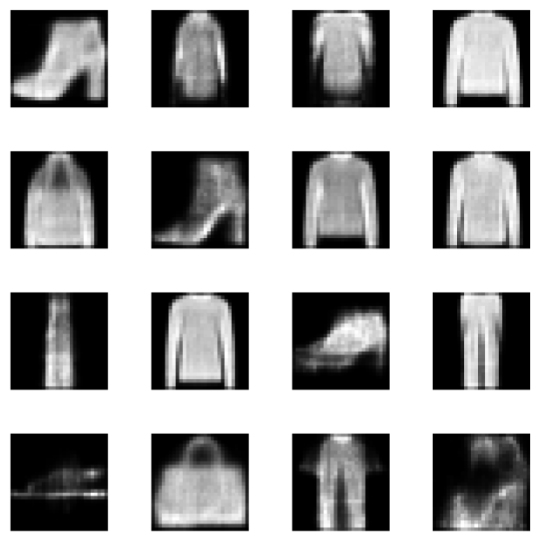
\includegraphics[width=7cm]{./VAE.png}
   \caption{VAEが生成した画像データ}
   \label{fig:}
 \end{center}
\end{figure}

\section{GAN}
VAEは生成した画像がぼやけてしまうが, これは学習が足りてないのではなくモデルの枠組み, 学習の仕方に原因がある. VAEでは, 生成モデルを正規分布あるいはベルヌーイ分布として明示的にモデル化し, 最尤推定により学習を行っていた. これにより, 誤差関数には2乗誤差あるいは交差エントロピー誤差の項が用いられることになるが, これを最小化しようとすると, 全体的に画素を曖昧にさせた方が画像全体として誤差は小さくなるので, VAEではどうしても生成画像がぼやける傾向が出てしまう. これを改善するために生成モデルの分布をモデルを暗黙的にするGANが考えられた.
データ分布を${p_d(x)}$, データ分布に近いモデル分布を${p_g(x)}$とおく. ここでは分布${p_d(x)}$は分布の形が明示されていない. そのため尤度を測ることもできないので, まずはデータ分布とモデル分布の密度比${r(x)}$を考える.
\begin{equation}
  r(x) = \frac{p_d(x)}{p_g(x)}
\end{equation}
ここで, データ分布あるいはモデル分布から生成されたラベル付きのデータ集合${\{(x_1, y_1), \ldots, (x_N, y_N)\}}$を考え, データ分布により生成されたデータのラベルを${y=1}$, モデル分布により生成されたデータのラベルを${y=0}$とすると, それぞれの分布は次のようになる.
\begin{eqnarray}
  p_d(x) = p(x|y=1) \\
  p_g(x) = p(x|y=0)
\end{eqnarray}
この時, 密度比${r(x)}$は次のように変形できる.
\begin{eqnarray}
  r(x) &=& \frac{p(x|y=1)}{p(x|y=0)} \nonumber \\
  &=& \frac{p(y=1)p(x)}{p(y=1)} \frac{p(y=0)}{p(y=0|x)p(x)} \nonumber \\
  &=& \frac{p(y=1|x)}{p(y=0|x)} \frac{1-\pi}{\pi}
\end{eqnarray}
ただし,
\begin{equation}
  \pi = p(y=1)
\end{equation}
である.${p(y=1|x)}$を推定することができれば, ${r(x)}$がもとまるので ${p(y=1|x)}$を近似する分布をパラメータ${\phi}$を用いて${p_\phi(y=1|x)}$とする.
\begin{equation}
  p(y=1|x) \simeq q_\phi(y=1|x)
\end{equation}
こうすることで, 分布をNNで求めることができるようになる. この${q_\phi(y=1|x)}$を推定するモデルのことを{\bf 識別器}あるいは{\bf 鑑別器(discriminator)}という. 識別器を${D(\phi;x)}$と表す.
\begin{equation}
  D(\phi;x) = q_\phi(y=1|x)
\end{equation}
これにより, 密度比を考える問題から, 確率的分類器の最適化, すなわち一般的な分類問題に置き換わったことになる. よって誤差関数として, 交差エントロピー誤差関数を考えると,
\begin{equation}
  \U(D) = -E_{p(x, y)} [y\ln D(\phi; x) + (1 - y)\ln(1 - D(\phi; x))]
\end{equation}

と表せる. 符号の煩わしさから${-U(D)}$を考え, 次のように式変形を行うと
\begin{eqnarray}
  && E_{p(x, y)} [y\ln D(\phi; x) + (1 - y)\ln(1 - D(\phi; x))] \nonumber \\
  &=& E_{p(x|y)p(y)} [y\ln D(\phi; x) \nonumber \\
   && + (1 - y)\ln(1 - D(\phi; x))] \nonumber \\
  &=& E_{p(x|y=1)p(y=1)}[\ln D(\phi;x)] \nonumber \\
  && + E_{p(x|y=0)p(y=0)}[\ln (1 - D(\phi;x))] \nonumber \\
  &=& \pi E_{p_d (x)}[\ln D(\phi;x)] \nonumber \\
  &&+ (1 - \pi) E_{p_g(x)}[\ln (1 - D(\phi; x))]
\end{eqnarray}
ここで, データ集合に関して, 各ラベルのデータが等しい時
\begin{equation}
  \pi = 1 - \pi = \frac{1}{2}
\end{equation}
であるから, 最終的な識別器の目的関数${V(D)}$は
\begin{equation}
  V(D) = E_{p_d(x)}[\ln D(\phi;x)] + E_{p_g(x)}[\ln (1 - D(\phi;x))]
\end{equation}
で, 識別器の目的はこれを最大化することである. もし, 最適な識別器 ${D_\ast(\phi;x)}$が得られたとすると,
\begin{equation}
  D_\ast(\phi;x) = D_\ast(x) = p(y = 1 | x)
\end{equation}
となるが, この時
\begin{equation}
  D_\ast(x) = \frac{r}{r + 1} = \frac{p_d(x)}{p_d(x) + p_g(x)}
\end{equation}
に収束する. これを目的関数${V(D)}$に代入すると,
\begin{eqnarray}
  V(D_\ast) &=& E_{p_d} [\ln \frac{p_d}{p_d + p_g}] + E_{p_g} [\ln (1 - \frac{p_d}{p_d + p_g})] \nonumber \\
  &=& \int_{}^{} p_d \ln \frac{p_d}{p_g} \,\mathrm{d}x  + \int_{}^{} p_g \ln \frac{p_g}{p_d + p_g} \,\mathrm{d}x \nonumber \\
  &=& \int_{}^{} p_d \ln \frac{2p_d}{p_d + p_g} \,\mathrm{d}x  - \int_{}^{} p_d \ln 2 \,\mathrm{d}x \nonumber \\
  &&+ \int_{}^{} p_g \ln \frac{2p_g}{p_d + p_g} \,\mathrm{d}x - \int_{}^{} p_g \ln 2 \,\mathrm{d}x \nonumber \\
  &=& \int_{}^{} p_d \ln \frac{2p_d}{p_d + p_g} \,\mathrm{d}x \int_{}^{} p_g \ln \frac{2p_g}{p_d + p_g} \,\mathrm{d}x \nonumber \\
  &&- 2\ln 2 \nonumber \\
  &=& 2D_{JS}[p_d||p_g] - 2\ln2
\end{eqnarray}
つまり, ${V(D_\ast)}$は${p_d(x)}$と${p_g(x)}$のJSダイバージェンスに対応している. ここで, のJSダイバージェンスとは, KLダイバージェンスを${D_{KL}}$とすると
\begin{equation}
  D_{JS}[p||q] = \frac{1}{2}D_{KL}[p||\frac{p+q}{2}] + \frac{1}{2}D_{KL}[q||\frac{p+q}{2}]
\end{equation}
で定義されるものである.

次に生成モデルについて考える. 潜在変数${z}$を仮定すると, 周辺化により
\begin{equation}
  p_g(x) = \int_{}^{} p(x|z)p(z)\,\mathrm{d}z
\end{equation}
となるが, 今度は${p(z|x)}$を近似する分布として${q_\theta(x|z)}$を導入する.
\begin{equation}
  p(x|z) \simeq q_\theta(x|z)
\end{equation}
こうすることで, この分布をNNで求められる. 生成器を${G(\theta;z)}$で表すと,
\begin{equation}
  G(\theta;z) = q_\theta(x|z)
\end{equation}
と表す. 最適な${G(\theta;z)}$を得るための目的関数は, ${D_\ast}$を用いて
\begin{equation}
  V(D_\ast, G) = E_{p_d(x)}[\ln D_\ast(x)] + E_{p(z)}[\ln(1 - D_\ast(G(\theta; z)))]
\end{equation}
と表せ, 生成器は${V(D_\ast, G)}$を最小化する.

\subsection{まとめ}
以上をまとめると, GANは以下の識別器の学習と生成器の学習を片方を固定して交互に行うことになる. 識別器の学習は, 生成器${G(\theta;z)}$を固定した上で,
\begin{equation}
  \max_\theta E_{p_d(x)}[\ln D(\phi; x)] + E_{p(z)}[\ln (1 - D(\phi; G(\theta; z)))]
\end{equation}
を計算し, 生成器の学習は, 識別器${D(\phi;x)}$を固定した上で
\begin{equation}
  \min_\theta E_{p(z)} [\ln (1 - D(\theta; G(\theta; z)))]
\end{equation}
を計算する.


\begin{thebibliography}{9}
  \bibitem{論文} Generative Adversarial Nets https://arxiv.org/pdf/1406.2661.pdf
  \bibitem{サイト} 巣籠悠輔. 詳説ディープラーニング(生成モデル編) https://note.com/yusugomori/n/n945f51cabc03
\end{thebibliography}
\end{document}
